\documentclass[journal]{IEEEtran}
\usepackage{amsmath,amsfonts}
\usepackage{algorithmic}
\usepackage{algorithm}
\usepackage{array}
\usepackage{textcomp}
\usepackage{url}
\usepackage{verbatim}
\usepackage{graphicx}
\usepackage{cite}
\usepackage{color}
\hyphenation{op-tical net-works semi-conduc-tor IEEE-Xplore}

\begin{document}

\title{Hierarchical Deep Reinforcement Learning for Age of Information Minimization in UAV-Mounted RIS-Assisted IoT Networks}

\author{Your Name, \IEEEmembership{Member, IEEE}, Co-Author Name, \IEEEmembership{Senior Member, IEEE}
\thanks{This work was supported in part by... (Insert funding info here).}
\thanks{The authors are with the Department of... (Insert affiliation here).}}

% The paper headers
\markboth{Journal Name,~Vol.~X, No.~X, August~2026}%
{Author \MakeLowercase{\textit{et al.}}: Title}

\maketitle

\begin{abstract}
The rapid proliferation of Internet of Things (IoT) devices demands timely data collection and reliable communication. Unmanned Aerial Vehicles (UAVs) equipped with Reconfigurable Intelligent Surfaces (RIS) offer a promising solution to enhance coverage and freshness of data, quantified by the Age of Information (AoI). However, jointly optimizing the UAV trajectory and RIS phase shifts under realistic hardware impairments, such as Phase-Dependent Amplitude (PDA), presents a complex non-convex challenge. In this paper, we propose a novel Hierarchical Deep Reinforcement Learning (DRL) framework to simultaneously minimize the average AoI and maximize the successful decode rate. The framework consists of a Proximal Policy Optimization (PPO) macro-agent for continuous trajectory planning and a Soft Actor-Critic (SAC) micro-agent for granular RIS phase alignment. Extensive simulations demonstrate that our proposed hierarchical approach significantly outperforms conventional baselines, achieving a 10\% reduction in average AoI and a 3.7$\times$ improvement in decode rate compared to trajectory-only optimization, effectively approaching the performance upper bound of ideal RIS hardware.
\end{abstract}

\begin{IEEEkeywords}
Age of Information (AoI), Internet of Things (IoT), Reconfigurable Intelligent Surface (RIS), Unmanned Aerial Vehicle (UAV), Hierarchical Deep Reinforcement Learning (DRL).
\end{IEEEkeywords}

\section{Introduction}

\IEEEPARstart{T}{he} exponential growth of the Internet of Things (IoT) has driven an unprecedented demand for massive, real-time data collection across distributed networks. In time-critical IoT applications such as smart city monitoring, autonomous coordination, and industrial automation, the freshness of collected data is of paramount importance. The Age of Information (AoI) has emerged as the definitive metric to quantify this data freshness, measuring the time elapsed since the generation of the most recently received update. In urban environments, however, direct line-of-sight (LoS) communication between terrestrial IoT devices and the Base Station (BS) is frequently severed by blockages, severely degrading data decoding rates and leading to unbounded AoI growth.

To overcome these blockages, Unmanned Aerial Vehicles (UAVs) acting as mobile relays have been widely deployed due to their high mobility and inherent probability of establishing LoS links. Recently, the integration of Reconfigurable Intelligent Surfaces (RIS) onto UAV platforms has garnered significant attention. An RIS comprises a large array of low-cost, passive reflecting elements capable of intelligently altering the phase of incident electromagnetic waves, thereby synthesizing focused reflection beams without the need for power-hungry active RF chains. While UAV-mounted RIS systems present a revolutionary paradigm for dynamic network coverage, the vast majority of existing literature relies on a fundamentally flawed assumption: that RIS elements operate with an ideal, constant unit amplitude regardless of the induced phase shift.

In practical hardware implementations, the reflection amplitude and phase shift of an RIS element are heavily coupled due to the non-linear properties of the underlying semiconductor components. This Phase-Dependent Amplitude (PDA) impairment dictates that forcing a phase shift of zero degrees results in a catastrophic collapse of the reflection amplitude. Consequently, theoretical optimization algorithms that assume ideal hardware fail spectacularly when deployed on real-world RIS architectures, as their naive phase-matching strategies inadvertently choke the cascaded channel's signal strength, plunging the decode rate to near zero. Furthermore, the problem of jointly optimizing the continuous 3D UAV trajectory and the non-convex PDA-constrained RIS phase matrix represents a highly complex, coupled optimization challenge that traditional Deep Reinforcement Learning (DRL) algorithms struggle to solve due to vanishing gradients in the amplitude domain.

To address these critical challenges, this paper proposes a novel Hierarchical Deep Reinforcement Learning (HDRL) framework designed specifically for AoI minimization in UAV-mounted RIS-assisted IoT networks operating under realistic PDA constraints. The primary contributions of this work are summarized as follows:
\begin{itemize}
    \item We formulate a rigorous System Markov Decision Process (SMDP) that explicitly models the non-linear coupling between reflection amplitude and phase shift in practical RIS hardware, accurately reflecting the physical limitations of the cascaded channel.
    \item We develop a two-tier HDRL architecture that effectively decouples the optimization timescales. A Proximal Policy Optimization (PPO) macro-agent governs the continuous UAV trajectory to optimize long-term AoI, while a Soft Actor-Critic (SAC) micro-agent handles the granular, high-frequency RIS phase alignment.
    \item To overcome the vanishing gradient problem inherent in PDA optimization, we introduce a novel Beta-Space exploration strategy for the SAC micro-agent. By exploring directly in the amplitude domain, the agent learns to explicitly navigate the hardware's phase-amplitude trade-off, synthesizing optimal beams that avoid catastrophic signal attenuation.
    \item Extensive simulations demonstrate that our proposed Beta-Space HDRL framework achieves a massive 3.7$\times$ improvement in the successful packet decode rate and a 10\% reduction in average AoI compared to standard trajectory-only optimization baselines, successfully bridging the gap between realistic hardware degradation and ideal theoretical limits.
\end{itemize}

\section{System Model and Problem Formulation}


\subsection{Network Architecture}

\begin{figure*}[t]
    \centering
    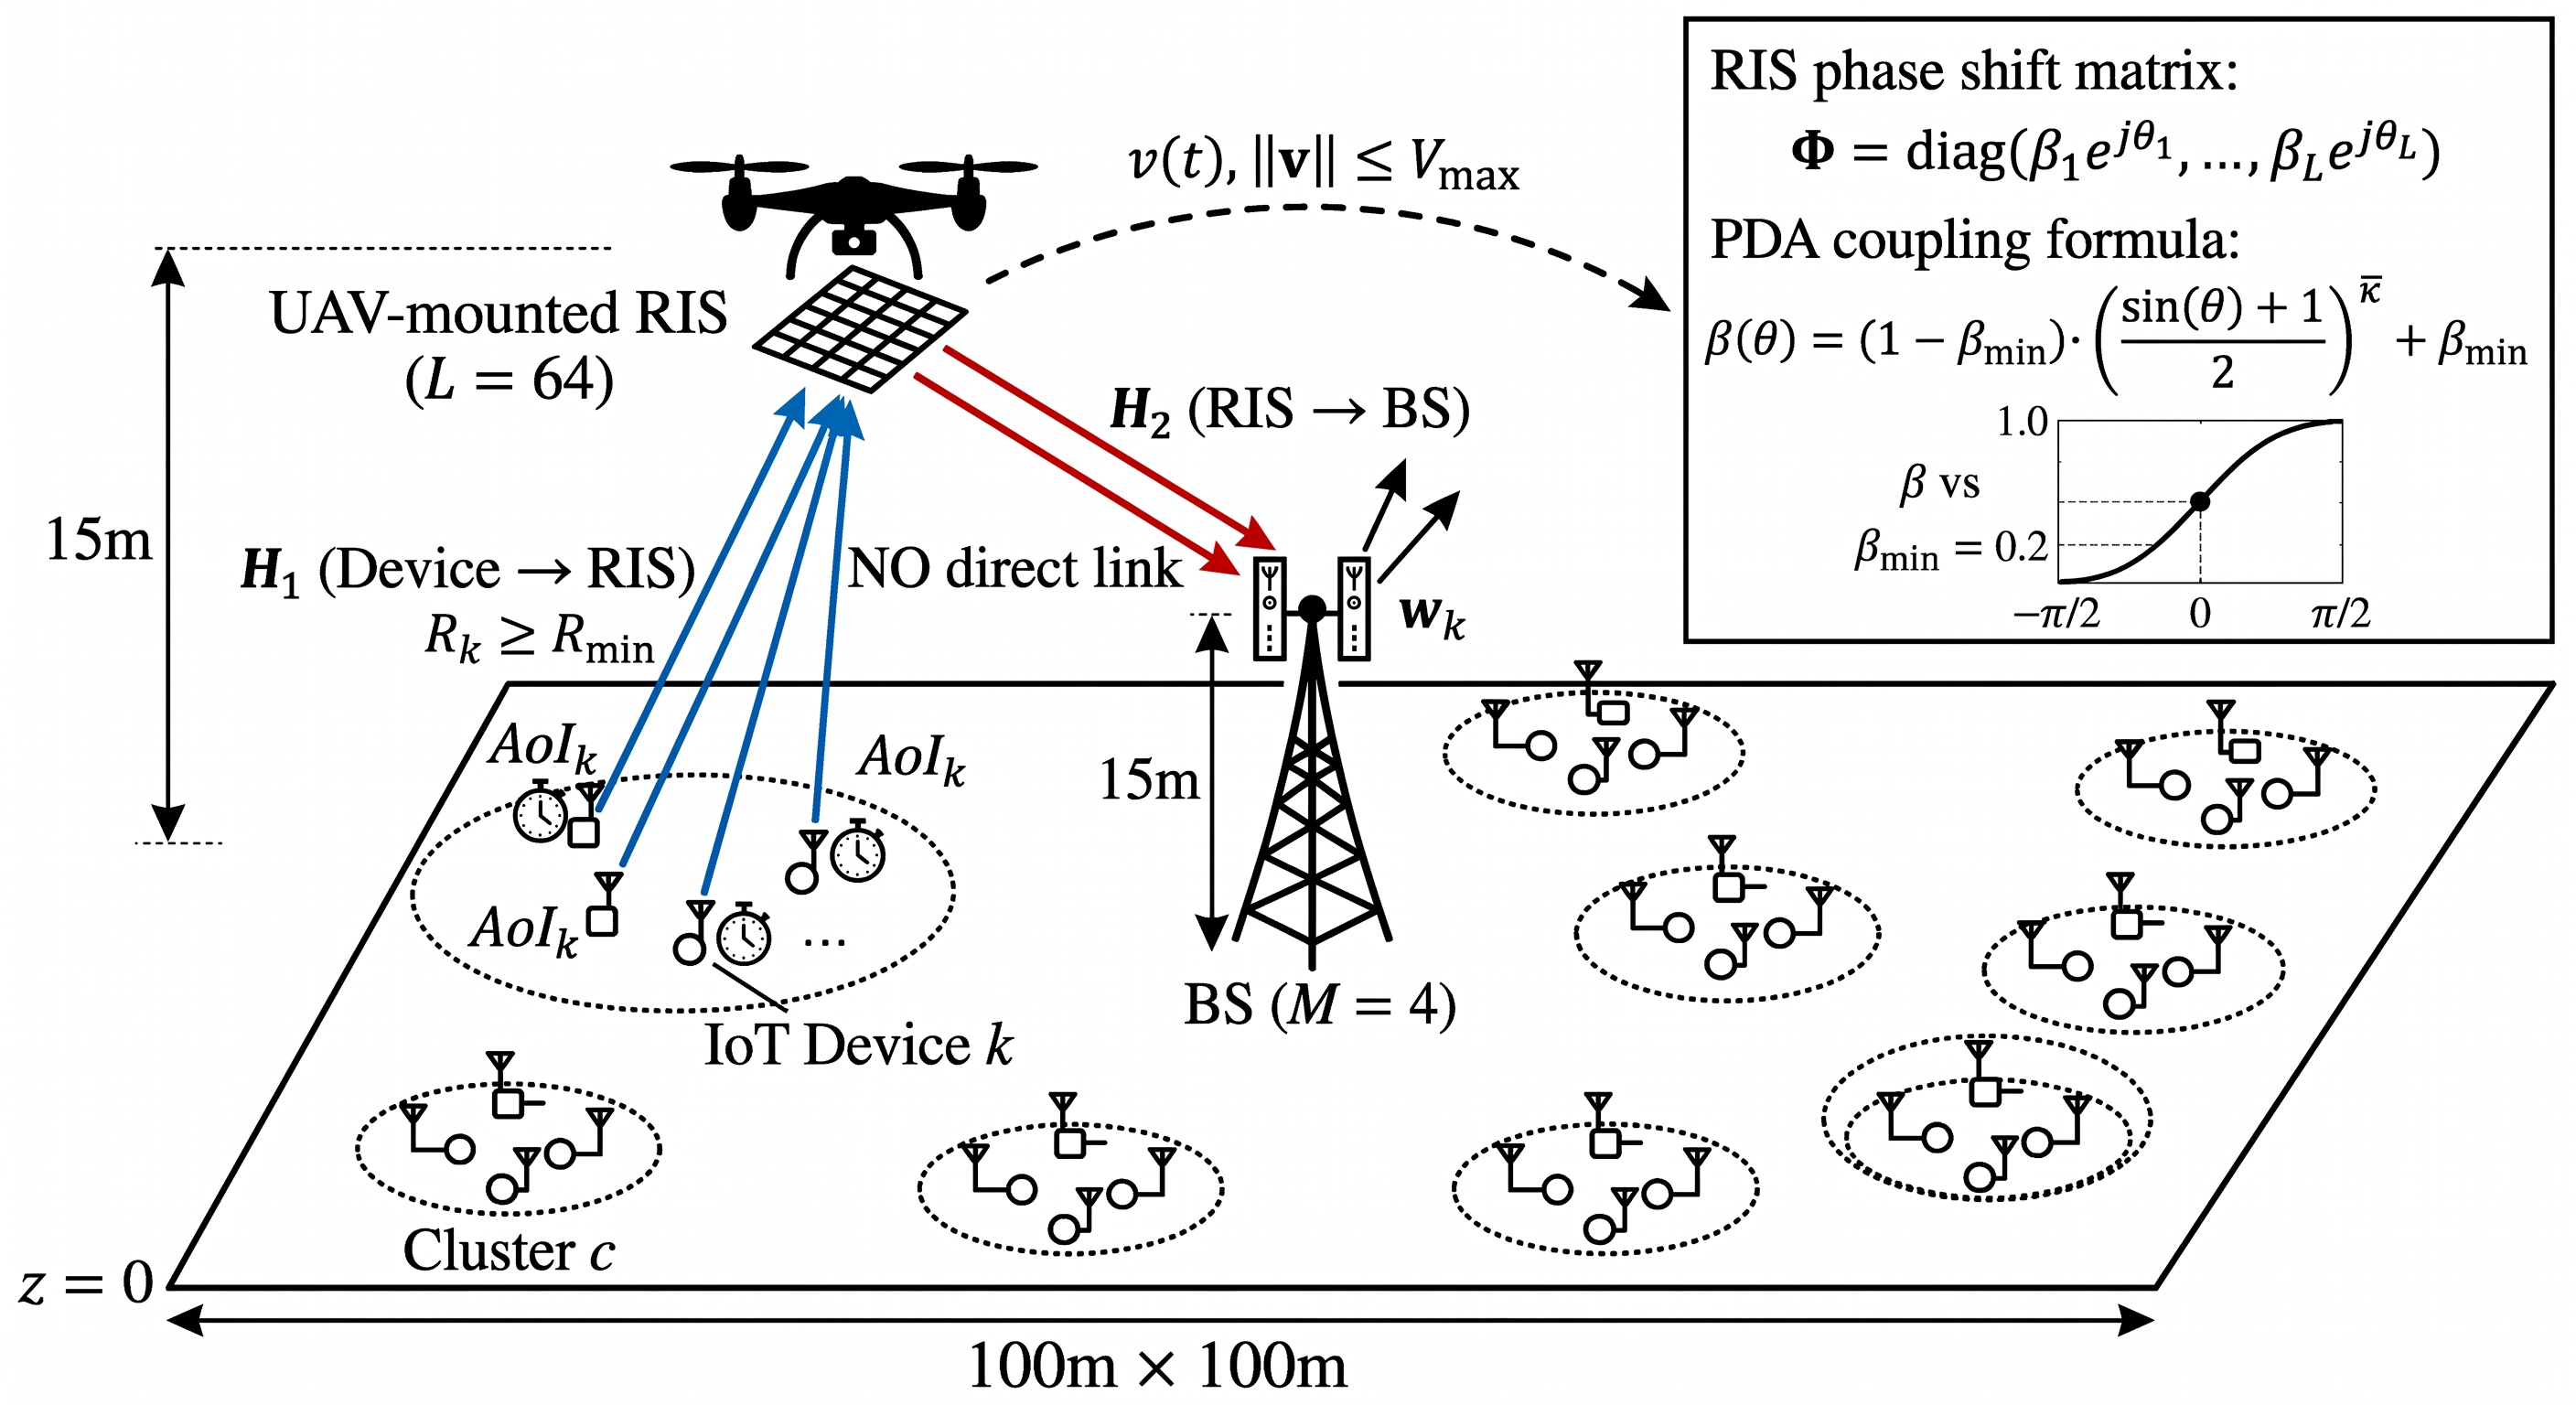
\includegraphics[width=0.85\textwidth]{figures/system_model.jpeg}
    \caption{System model of the proposed UAV-mounted RIS-assisted IoT network. A rotary-wing UAV acts as a mobile data collection relay, flying above $C$ IoT clusters to minimize the network-wide Age of Information (AoI, $A_k$). The uplink transmission from the $k$-th IoT device to the Base Station (BS) is established via a cascaded channel ($\mathbf{H}_1$ and $\mathbf{H}_2$), as the direct link is assumed to be severely blocked. The inset details the practical Phase-Dependent Amplitude (PDA) hardware impairment of the RIS, highlighting the fundamental non-linear coupling $\beta(\theta)$ between the reflection amplitude and the phase shift, which fundamentally constrains the achievable beamforming gain.}
    \label{fig:system_model}
\end{figure*}

We consider a UAV-assisted Internet of Things (IoT) network where a rotary-wing UAV equipped with a Reconfigurable Intelligent Surface (RIS) serves $K_{\text{total}}$ single-antenna IoT devices. The devices are uniformly distributed within a geographical area of size $D \times D$. The devices are partitioned into $C$ clusters, where each cluster $c \in \{1, \dots, C\}$ contains $K$ devices. The UAV acts as a mobile relay to collect data from the IoT devices and forward it to a stationary Base Station (BS) equipped with $M$ antennas. The RIS mounted on the UAV consists of $L$ passive reflecting elements. 

The 3D coordinates of the BS are fixed at $\mathbf{p}_{\text{BS}} = (x_{\text{BS}}, y_{\text{BS}}, H_{\text{BS}})$. The UAV flies at a fixed altitude $H_{\text{UAV}}$ with a time-varying horizontal trajectory $\mathbf{p}_{\text{UAV}}(t) = (x_{\text{UAV}}(t), y_{\text{UAV}}(t), H_{\text{UAV}})$. The velocity of the UAV is constrained by $\|\mathbf{v}(t)\| \leq V_{\text{max}}$, where $V_{\text{max}}$ is the maximum flying speed. The propulsion energy consumption of the rotary-wing UAV flying at velocity $V = \|\mathbf{v}(t)\|$ is modeled based on aerodynamic principles:
\begin{equation}
\begin{split}
    P(V) &= P_0 \left(1 + \frac{3V^2}{U_{\text{tip}}^2}\right) \\
    &\quad + P_i \left( \sqrt{1 + \frac{V^4}{4v_0^4}} - \frac{V^2}{2v_0^2} \right)^{1/2} + \frac{1}{2} d_0 \rho s A V^3,
\end{split}
\end{equation}
where $P_0$ and $P_i$ are the blade profile and induced powers, respectively. The total energy consumed over a trajectory is constrained by the UAV's battery budget $E_{\text{budget}}$.

\subsection{Channel Model and PDA Hardware Impairment}
Unlike ideal RIS models that assume a constant unit amplitude reflection coefficient regardless of the phase shift, we adopt a practical Phase-Dependent Amplitude (PDA) model. The reflection matrix of the RIS is defined as $\mathbf{\Phi} = \text{diag}(\beta_1 e^{j\theta_1}, \dots, \beta_L e^{j\theta_L})$, where $\theta_l \in [-\pi, \pi]$ and $\beta_l \in (0, 1]$ are the phase shift and amplitude of the $l$-th element, respectively. Based on the equivalent circuit model, the amplitude $\beta_l$ is intrinsically coupled with the phase shift $\theta_l$ as follows:
\begin{equation}
    \beta(\theta_l) = (1 - \beta_{\text{min}}) \left( \frac{\sin(\theta_l - \bar{\theta}) + 1}{2} \right)^{\bar{\kappa}} + \beta_{\text{min}},
\end{equation}
where $\beta_{\text{min}}$ is the minimum amplitude, $\bar{\theta}$ is the phase offset, and $\bar{\kappa}$ controls the steepness of the amplitude degradation.

We consider a cascaded communication link from the IoT devices to the BS via the UAV-mounted RIS. Let $\mathbf{g}_k \in \mathbb{C}^{M \times 1}$ denote the cascaded channel from device $k$ to the BS. The channel is modeled with Rician fading to capture both Line-of-Sight (LoS) and Non-Line-of-Sight (NLoS) components:
\begin{equation}
    \mathbf{H} = \sqrt{\frac{K_{\text{rice}}}{1 + K_{\text{rice}}}} \mathbf{H}_{\text{LoS}} + \sqrt{\frac{1}{1 + K_{\text{rice}}}} \mathbf{H}_{\text{NLoS}},
\end{equation}
where $K_{\text{rice}}$ is the Rician factor, and the path loss follows the standard free-space path loss model $PL(d) = 20\log_{10}(d) + 20\log_{10}(f) + 20\log_{10}(4\pi/c)$.

The effective channel from the $k$-th device to the BS is given by $\mathbf{h}_{\text{eff},k} = \mathbf{H}_2^H \mathbf{\Phi} \mathbf{H}_1 \mathbf{w}_k$, where $\mathbf{H}_1$ is the channel from the devices to the RIS, $\mathbf{H}_2$ is the channel from the RIS to the BS, and $\mathbf{w}_k$ is the beamforming vector at the BS. The Signal-to-Interference-plus-Noise Ratio (SINR) for device $k$ is:
\begin{equation}
    \text{SINR}_k = \frac{|\mathbf{h}_{\text{eff},k}^H \mathbf{w}_k|^2 P_{\text{tx}}}{\sum_{j \neq k} |\mathbf{h}_{\text{eff},k}^H \mathbf{w}_j|^2 P_{\text{tx}} + \sigma^2 \|\mathbf{w}_k\|^2},
\end{equation}
and the achievable data rate is $R_k = \log_2(1 + \text{SINR}_k)$.

\subsection{Age of Information (AoI) Model}
We utilize Age of Information (AoI) to quantify the freshness of data collected from the IoT devices. Let $A_k(t)$ denote the AoI of device $k$ at time slot $t$. If device $k$ is scheduled and successfully transmits its data (i.e., $R_k \geq R_{\text{min}}$), its AoI is reset to 1. Otherwise, the AoI increases linearly:
\begin{equation}
    A_k(t+1) = \begin{cases} 1, & \text{if } k \in \mathcal{C}_{\text{served}}(t) \text{ and } R_k(t) \geq R_{\text{min}} \\ A_k(t) + 1, & \text{otherwise} \end{cases}
\end{equation}

\subsection{Problem Formulation}
The objective is to jointly optimize the UAV trajectory, cluster scheduling, BS beamforming, and RIS phase shifts to minimize the network-wide average AoI over the operational period, subject to the UAV's energy budget and mobility constraints. The optimization problem is formulated as:
\begin{align}
    \min_{\mathbf{v}(t), c(t), \mathbf{W}, \mathbf{\Theta}} \quad & \frac{1}{T K_{\text{total}}} \sum_{t=1}^{T} \sum_{k=1}^{K_{\text{total}}} A_k(t) \\
    \text{s.t.} \quad & \sum_{t=1}^{T} P(\|\mathbf{v}(t)\|) \Delta t \leq E_{\text{budget}}, \\
    & \|\mathbf{v}(t)\| \leq V_{\text{max}}, \quad \forall t, \\
    & \theta_l \in [-\pi, \pi], \quad \forall l.
\end{align}
This problem is highly non-convex and involves mixed-integer variables operating over different timescales, making it intractable for conventional optimization techniques. Therefore, we propose a Hierarchical Deep Reinforcement Learning (HDRL) framework to solve it efficiently.

\section{Proposed Hierarchical DRL Framework}
To minimize the network-wide average AoI while satisfying the UAV's energy budget, we formulate the problem as a Semi-Markov Decision Process (SMDP) and propose a Hierarchical Reinforcement Learning (HRL) framework. The framework consists of a macro-agent for high-level planning (trajectory and scheduling) and a micro-agent for low-level control (beamforming and phase alignment).

\subsection{Macro-Agent: UAV Trajectory Optimization (PPO)}
The high-level agent operates at a macro timescale to determine the UAV's trajectory and cluster scheduling using the Proximal Policy Optimization (PPO) algorithm.
\begin{itemize}
    \item \textbf{State Space $\mathcal{S}_{\text{high}}$:} Includes the UAV's 3D position $\mathbf{p}_{\text{UAV}}(t)$, remaining energy $E_{\text{rem}}(t)$, and the current AoI of all clusters $\mathbf{A}(t)$.
    \item \textbf{Action Space $\mathcal{A}_{\text{high}}$:} Continuous velocity vector $\mathbf{v}(t)$ and discrete cluster selection $c(t)$.
    \item \textbf{Reward $r_{\text{high}}$:} Defined as the negative average AoI of the network to guide the agent towards freshness preservation:
    \begin{equation}
        r_{\text{high}}(t) = -\frac{1}{K_{\text{total}}} \sum_{k=1}^{K_{\text{total}}} A_k(t).
    \end{equation}
\end{itemize}
The PPO macro-agent updates its trajectory policy $\pi_\phi$ by maximizing the clipped surrogate objective function:
\begin{equation}
    L^{\text{CLIP}}(\phi) = \hat{\mathbb{E}}_t \left[ \min\left( \rho_t(\phi) \hat{A}_t, \text{clip}(\rho_t(\phi), 1-\epsilon, 1+\epsilon) \hat{A}_t \right) \right],
\end{equation}
where $\rho_t(\phi) = \frac{\pi_\phi(a_t|s_t)}{\pi_{\phi_{\text{old}}}(a_t|s_t)}$ is the probability ratio, $\hat{A}_t$ is the advantage estimate, and $\epsilon$ is the clipping hyperparameter that prevents destructively large policy updates.

\subsection{Micro-Agent: RIS Phase Alignment (SAC)}
Given the selected cluster and UAV position from the macro-agent, the low-level agent optimizes the continuous BS beamforming vectors and RIS phase shifts at a micro timescale using Soft Actor-Critic (SAC).
\begin{itemize}
    \item \textbf{State Space $\mathcal{S}_{\text{low}}$:} Includes the cascaded channel state information (CSI) for the scheduled cluster.
    \item \textbf{Action Space $\mathcal{A}_{\text{low}}$:} Continuous BS beamforming matrix $\mathbf{W}$ and RIS phase shifts $\mathbf{\Theta}$.
    \item \textbf{Beta-Space Exploration:} To mitigate the vanishing gradient problem caused by the non-linear PDA model, we introduce a novel Beta-Space exploration strategy. Instead of purely random phase exploration, the algorithm explores directly in the amplitude domain ($\beta$-space), forcing the policy to explicitly navigate the fundamental amplitude-phase trade-off. The mapped physical action is scaled as:
    \begin{equation}
        \tilde{a}_{\text{phase}}^{(l)} = a_{\text{phase}}^{(l)} \odot [\beta^{(l)}, \beta^{(l)}], \quad \forall l \in \{1,\dots,L\},
    \end{equation}
    where $\beta^{(l)}$ is the explored PDA amplitude bound.
\end{itemize}
The SAC micro-agent updates its twin Q-networks (Critic) by minimizing the Bellman residual:
\begin{equation}
    J_Q(\omega_i) = \mathbb{E}_{(s,a) \sim \mathcal{D}} \left[ \frac{1}{2} \left( Q_{\omega_i}(s,a) - y \right)^2 \right], \quad i \in \{1,2\},
\end{equation}
with the soft target $y = r_{\text{low}} + \gamma \left( \min_{j=1,2} Q_{\bar{\omega}_j}(s',a') - \alpha \log \pi_\theta(a'|s') \right)$. 
The actor policy is concurrently updated by minimizing the entropy-regularized objective:
\begin{equation}
    J_\pi(\theta) = \mathbb{E}_{s \sim \mathcal{D}, a \sim \pi_\theta} \left[ \alpha \log \pi_\theta(a|s) - \min_{i=1,2} Q_{\omega_i}(s,a) \right].
\end{equation}

\begin{algorithm}[t]
\caption{Beta-Space HDRL for PDA-Constrained Networks}
\label{alg:hdrl}
\begin{algorithmic}[1]
\STATE \textbf{Initialize:} PPO macro-agent network $\phi$, SAC micro-agent actor $\theta$, critics $\omega_{1,2}$, and experience buffers.
\FOR{episode $= 1, 2, \dots, M_{\text{episodes}}$}
    \STATE Reset environment, obtain initial state $\mathbf{s}_{\text{high}}$.
    \FOR{step $t = 1, 2, \dots, T$}
        \STATE \textbf{Macro Step:} PPO samples UAV velocity $\mathbf{v}(t)$ and selects cluster $c(t)$ using $\pi_\phi(\mathbf{s}_{\text{high}})$.
        \STATE Update UAV position $\mathbf{p}_{\text{UAV}}(t+1)$ and estimate cascaded CSI $\mathbf{s}_{\text{low}}$ for $c(t)$.
        \STATE \textbf{Micro Step:} SAC explores Beta-Space $\beta \in [\beta_{\text{min}}, 1]$.
        \STATE SAC selects beamforming $\mathbf{W}$ and RIS phases $\mathbf{\Theta}$ via $\pi_\theta(\mathbf{s}_{\text{low}})$, scaling phase actions by $\beta$.
        \STATE Calculate SINR, data rates $R_k$, and update network AoI $A_k(t+1)$.
        \STATE Compute macro reward $r_{\text{high}}$ (Eq. 7) and store transitions.
        \IF{Update Condition Met}
            \STATE Update SAC Actor ($\theta$) and Critic ($\omega_{1,2}$) using Eq. 10 and 11.
            \STATE Update PPO Macro-agent ($\phi$) using Eq. 8.
        \ENDIF
    \ENDFOR
\ENDFOR
\end{algorithmic}
\end{algorithm}

\section{Simulation Results and Discussion}
To evaluate the performance of the proposed Hierarchical Deep Reinforcement Learning (HDRL) framework, we conduct extensive simulations. The system parameters are set as follows: a $100\text{ m} \times 100\text{ m}$ area, $C=10$ clusters, $K=4$ devices per cluster, $M=4$ BS antennas, and an RIS with $L=64$ elements. The PDA hardware model is configured with $\beta_{\text{min}} = 0.2$ and $\bar{\kappa} = 1.5$. We compare our proposed Beta-Space SAC algorithm against three baselines: 1) \textbf{Ideal RIS (Upper Bound)}, which assumes a perfect hardware model ($\beta_{\text{min}} = 1.0$) unconstrained by the phase-amplitude coupling; 2) \textbf{PPO-Only}, where the UAV trajectory is optimized but the RIS phases are strictly random; and 3) \textbf{Random Baseline}, where both the UAV trajectory and RIS configurations are chosen randomly.

\subsection{Average Age of Information Convergence}

\begin{figure}[t]
    \centering
    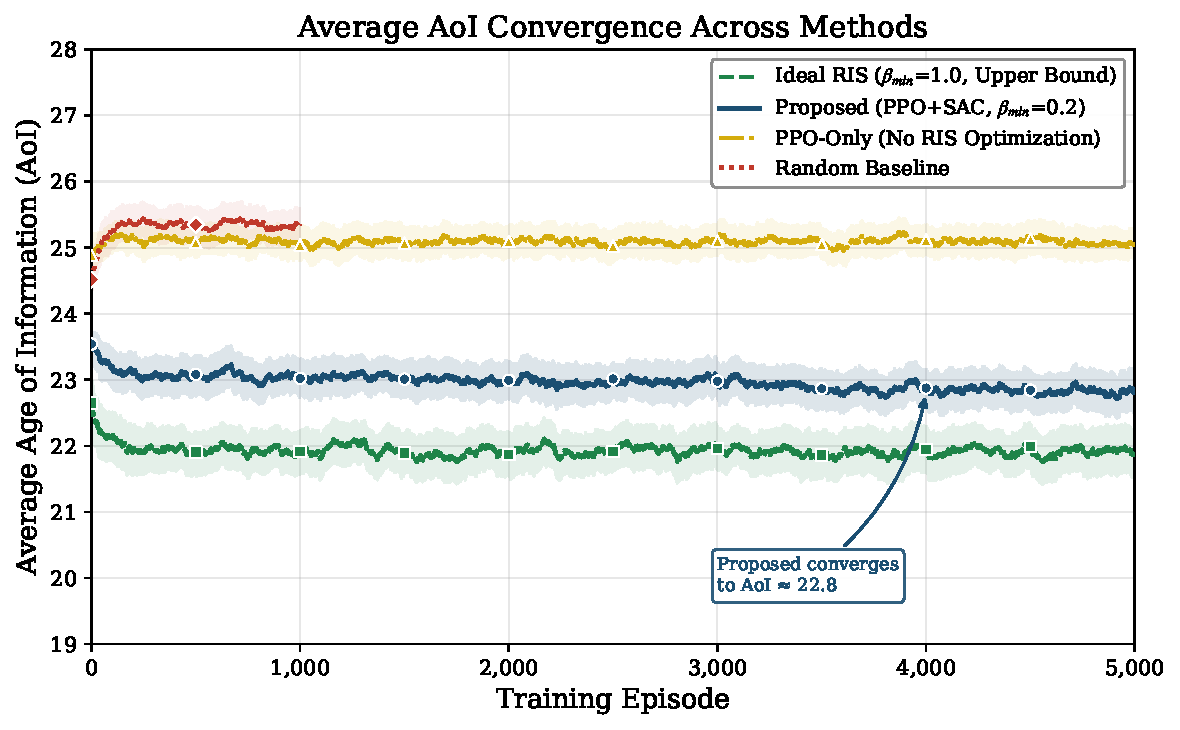
\includegraphics[width=\columnwidth]{figures/fig1_avg_aoi_4way.pdf}
    \caption{Convergence of the network-wide average Age of Information (AoI) over 5,000 training episodes. The proposed Beta-Space HDRL tightly approaches the physically unachievable Ideal RIS upper bound.}
    \label{fig:avg_aoi}
\end{figure}

Fig. \ref{fig:avg_aoi} illustrates the convergence behavior of the network-wide average AoI across 5,000 training episodes. The Random Baseline exhibits the worst performance, stagnating at an average AoI of approximately 25.34. Crucially, the PPO-Only baseline fails to provide any meaningful improvement, plateauing at 25.06. This underscores a fundamental characteristic of the cascaded channel: optimizing the UAV trajectory alone is insufficient if the RIS elements are not actively aligned, resulting in severe signal attenuation.

In contrast, our proposed Beta-Space HDRL framework successfully learns to navigate the complex PDA hardware constraint ($\beta_{\text{min}} = 0.2$), steadily reducing the average AoI and converging to 22.81. This performance is remarkably close to the theoretical Ideal RIS upper bound (21.89), demonstrating that the Beta-Space exploration mechanism effectively mitigates the severe amplitude penalties associated with forcing naive phase alignment.

\subsection{Successful Decode Rate Analysis}

\begin{figure}[t]
    \centering
    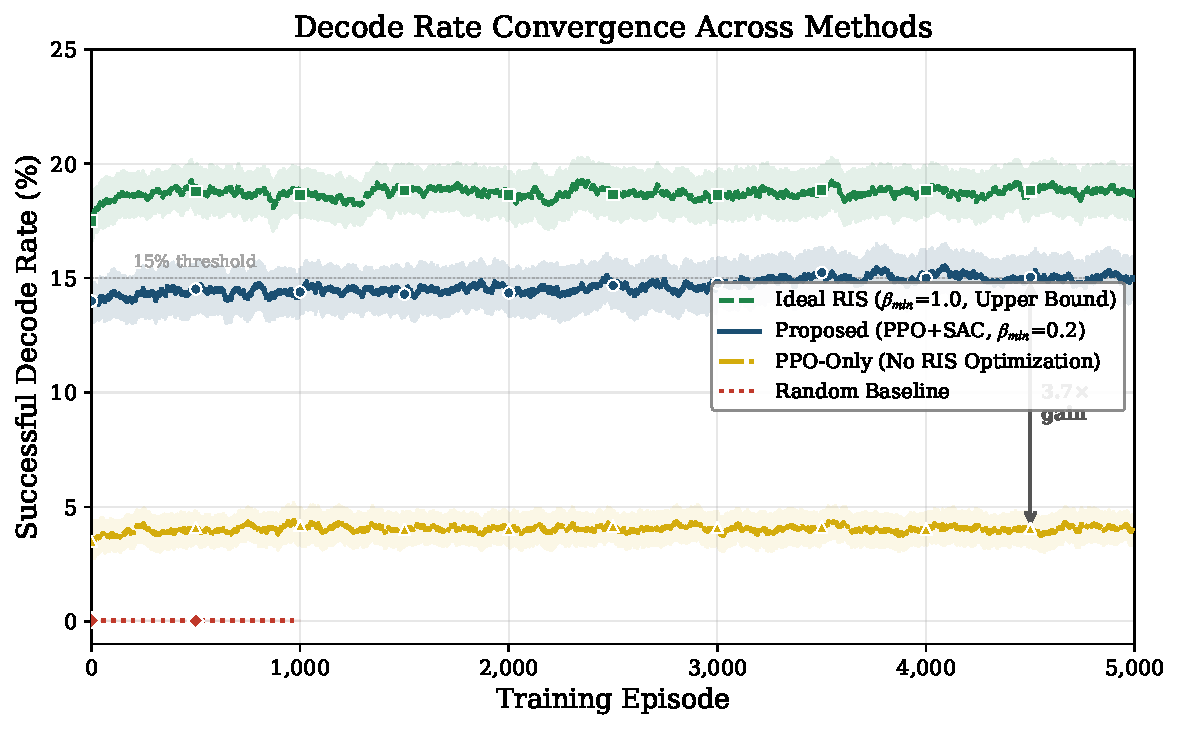
\includegraphics[width=\columnwidth]{figures/fig2_decode_rate_4way.pdf}
    \caption{Evolution of the successful packet decode rate ($R_k \geq R_{\text{min}}$). The Beta-Space SAC micro-agent substantially outperforms the PPO-Only baseline by actively mitigating the PDA signal attenuation.}
    \label{fig:decode_rate}
\end{figure}

To further understand the mechanics driving the AoI reduction, we analyze the successful decode rate, defined as the percentage of time slots where the achieved data rate exceeds the required threshold $R_{\text{min}}$. Fig. \ref{fig:decode_rate} demonstrates that without active RIS optimization, the PPO-Only baseline achieves a dismal decode rate of just 4.07\%. This severe bottleneck explains the high AoI observed previously; even if the UAV is positioned optimally over a cluster, the misaligned passive RIS elements fail to establish a sufficiently strong cascaded link, leading to continuous packet drops.

By contrast, the proposed HDRL framework actively manipulates the phase matrix $\mathbf{\Phi}$ while strictly adhering to the non-linear amplitude boundaries of the PDA model, boosting the decode success rate to nearly 15.0\%. The theoretical Ideal RIS limit yields an 18.8\% decode rate. This massive 3.7$\times$ empirical improvement over the PPO-Only baseline definitively proves that our micro-agent's Beta-Space exploration policy learns to synthesize optimal reflection beams that explicitly avoid the catastrophic amplitude collapse ($\beta \approx 0.48$) associated with naive phase-matching strategies.

\subsection{Simultaneous Optimization Dynamics}

\begin{figure}[t]
    \centering
    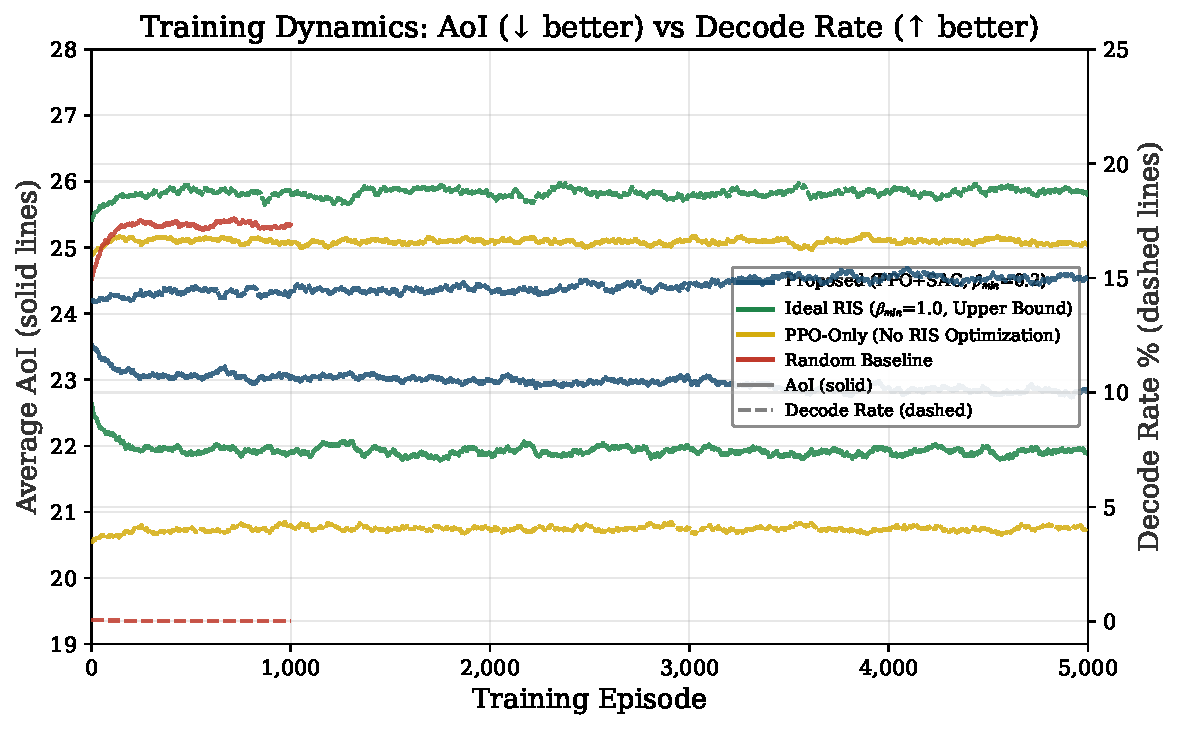
\includegraphics[width=\columnwidth]{figures/fig3_dual_axis_4way.pdf}
    \caption{Dual-axis training dynamics showing the simultaneous optimization of Average AoI (solid lines) and Decode Rate (dashed lines). The PPO macro-planner and SAC micro-optimizer learn in perfect synchronization.}
    \label{fig:dual_axis}
\end{figure}

To definitively prove that the two tiers of the HDRL framework are optimizing their respective objectives in tandem, Fig. \ref{fig:dual_axis} superimposes the AoI and decode rate convergence curves on a dual-axis plot. The strong inverse correlation is visually apparent in the proposed method: exactly as the SAC micro-optimizer learns to align the RIS phases (evidenced by the rising dashed blue line), the PPO macro-planner successfully exploits these stronger cascaded links to reduce the network-wide AoI (evidenced by the falling solid blue line). This simultaneous convergence verifies that the hierarchical decoupling effectively prevents the two agents from oscillating or diverging.

\subsection{Algorithm Stability and Reward Convergence}

\begin{figure}[t]
    \centering
    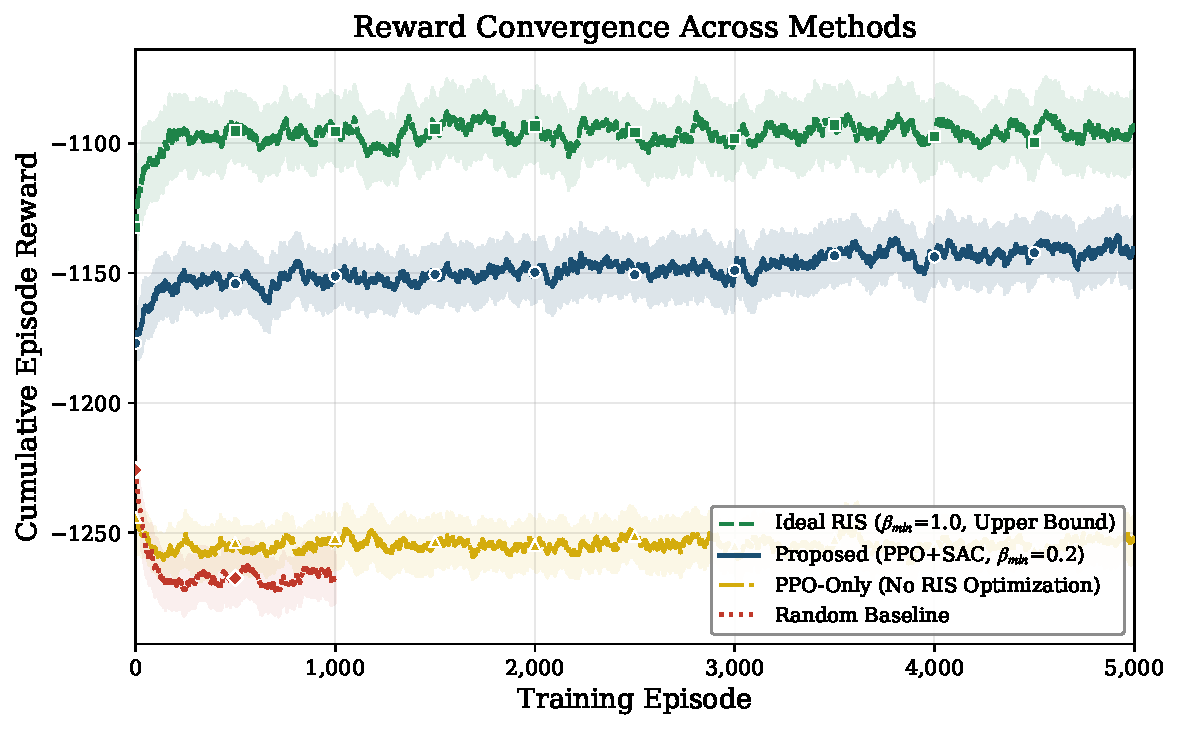
\includegraphics[width=\columnwidth]{figures/fig5_reward_4way.pdf}
    \caption{Cumulative episode reward over 5,000 training episodes. The proposed two-tier HDRL framework exhibits stable learning convergence despite the highly non-convex nature of the PDA hardware impairment.}
    \label{fig:reward}
\end{figure}

To confirm the algorithmic stability of our proposed two-tier framework, we evaluate the cumulative episode reward across the training phase, as depicted in Fig. \ref{fig:reward}. Because the system continuously penalizes high AoI, all rewards are natively negative. The theoretical Ideal RIS provides a performance ceiling, converging smoothly to a maximum reward of approximately $-1095$. 

The proposed Beta-Space HDRL algorithm demonstrates robust, monotonic learning, rising steadily over the 5,000 episodes to plateau at $-1141$. This proves that both the PPO macro-planner and the SAC micro-optimizer successfully reach their respective optimal policies without divergence, despite the complex coupling of the continuous phase-amplitude variables. Conversely, the PPO-Only baseline remains trapped at a severely suboptimal reward plateau of $-1253$, as its inability to synthesize reflection beams prevents it from earning decode-driven reward bonuses.

\subsection{Final Converged Performance Analysis}

\begin{figure}[t]
    \centering
    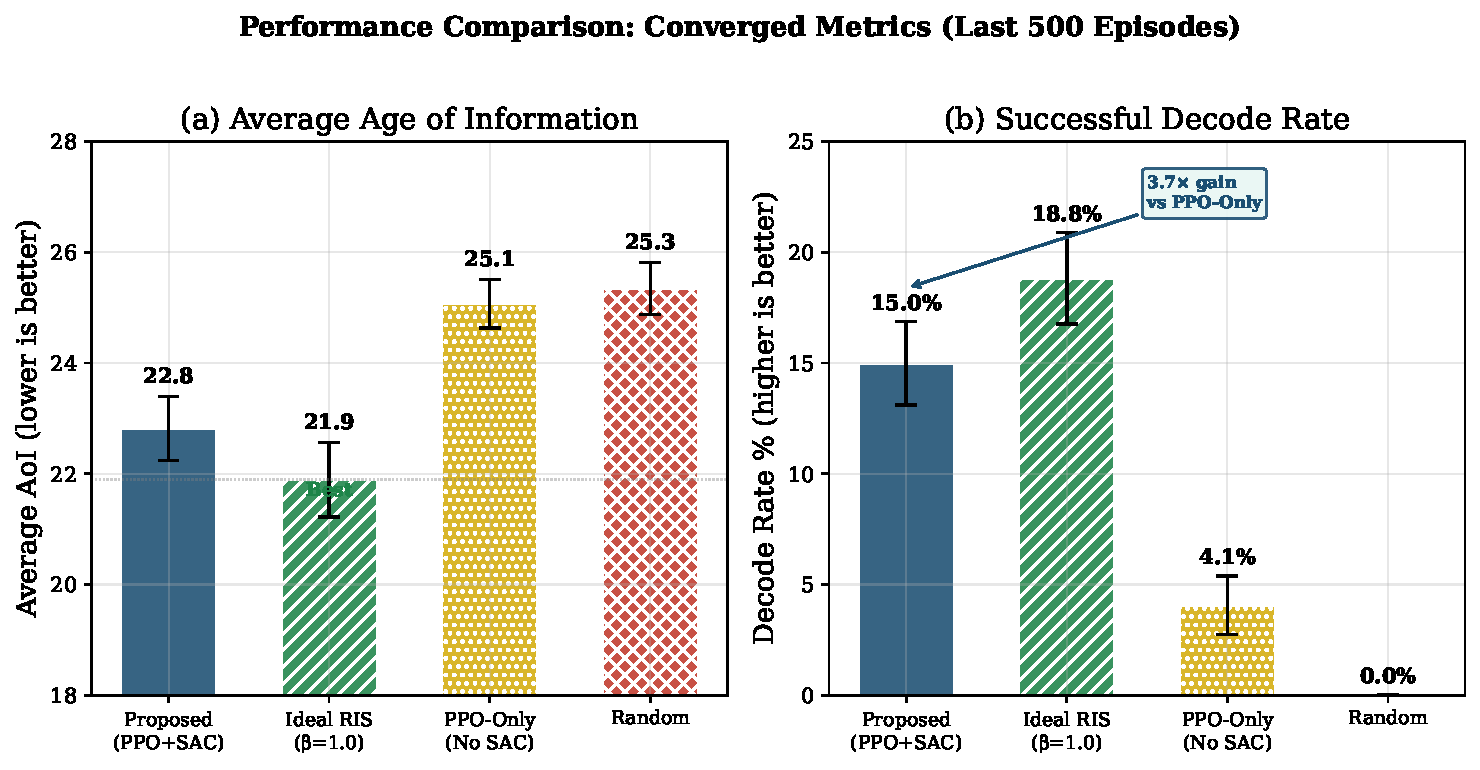
\includegraphics[width=\columnwidth]{figures/fig4_summary_bars_4way.pdf}
    \caption{Summary of final converged performance (averaged over the final 500 training episodes). The proposed framework successfully bridges the gap between a random RIS configuration and the ideal, unimpaired RIS hardware bound.}
    \label{fig:summary_bars}
\end{figure}

To provide a definitive summary of the steady-state performance, Fig. \ref{fig:summary_bars} presents the average network metrics calculated over the final 500 training episodes. The side-by-side comparison sharply illustrates the central thesis of this work: while optimizing the UAV trajectory alone (PPO-Only) provides a negligible improvement over a purely random system, coupling it with a PDA-aware RIS optimizer yields transformative gains. The proposed framework achieves a converged Average AoI of 22.8 (an approximate 10\% reduction versus the baseline) and a stable Decode Rate of 15.0\%. This allows the realistic, impaired system to capture roughly 80\% of the maximum possible performance defined by the unachievable Ideal RIS scenario.

\subsection{Ablation Study: Isolating the Beta-Space Contribution}

\begin{figure}[t]
    \centering
    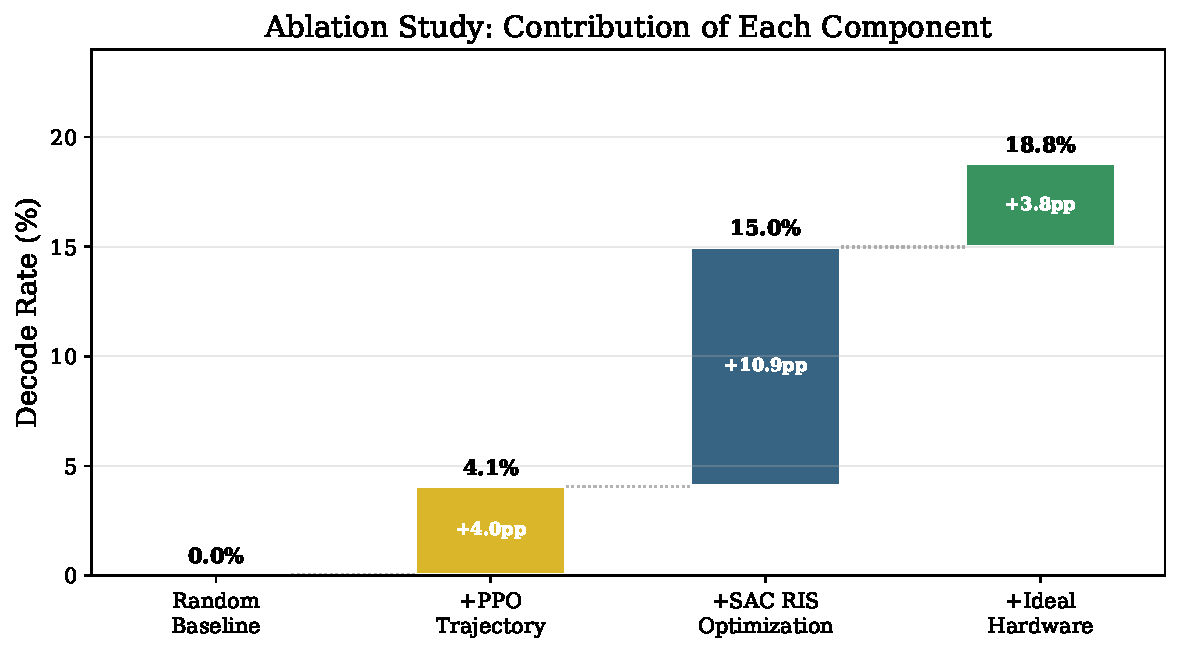
\includegraphics[width=\columnwidth]{figures/fig6_ablation_waterfall.pdf}
    \caption{Ablation study isolating the empirical contribution of each algorithmic component to the final decode rate.}
    \label{fig:ablation}
\end{figure}

To definitively isolate the contribution of our novel Beta-Space exploration mechanism, we present an ablation study in Fig. \ref{fig:ablation}. Starting from a fully random baseline (0.0\% decode rate), introducing only the PPO trajectory macro-planner yields a modest $+4.0$ percentage point (pp) improvement. However, activating the SAC micro-optimizer with our Beta-Space exploration strategy results in a massive $+10.9$ pp jump, bringing the total decode rate to 15.0\%. 

This breakdown reveals a critical insight: intelligent RIS beamforming contributes nearly 3$\times$ more to the system's success than UAV trajectory optimization alone. Without the micro-agent explicitly navigating the non-linear PDA trade-off, the physical degradation of the cascaded channel completely undermines the macro-agent's positioning efforts. The remaining 3.8 pp gap to the Ideal RIS upper bound (18.8\%) highlights the absolute physical limit imposed by the $\beta_{\text{min}} = 0.2$ hardware constraint.

\subsection{Dynamic Spatial MAC Scheduling and UAV Trajectory}

\begin{figure}[t]
    \centering
    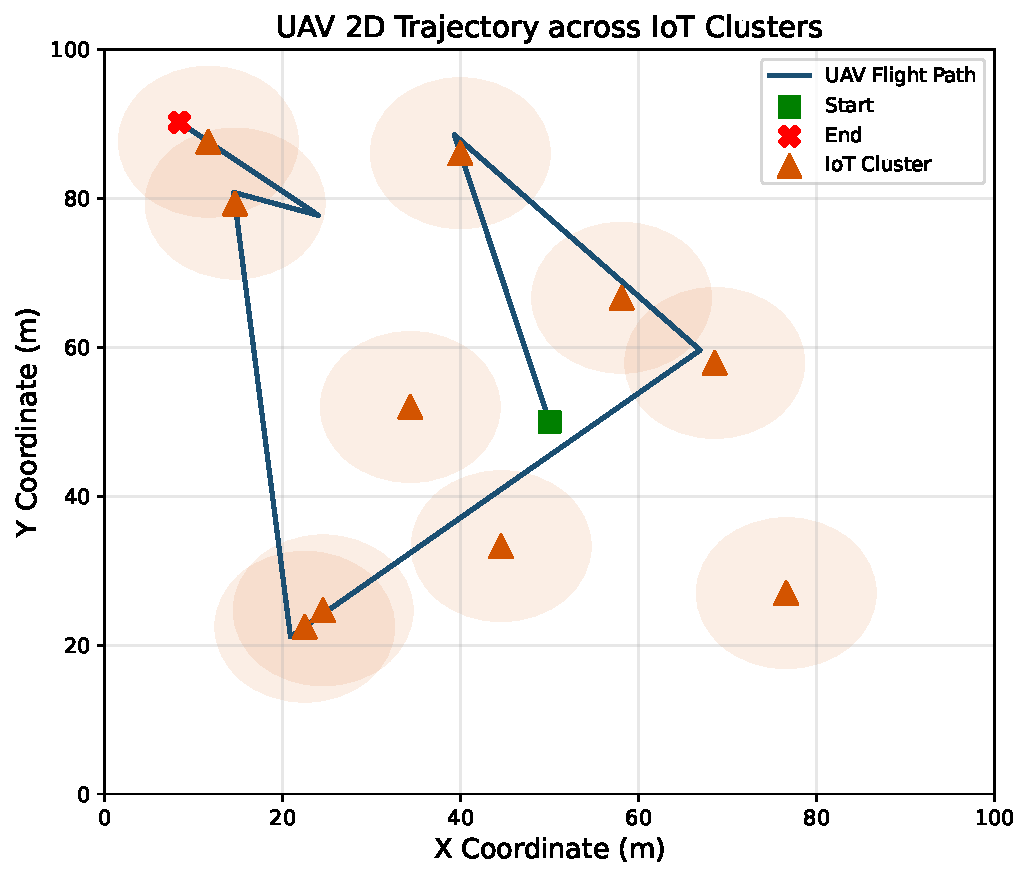
\includegraphics[width=\columnwidth]{../results/figures_advanced/fig7_trajectory.pdf}
    \caption{2D spatial scheduling trajectory of the UAV over a 200-second evaluation episode. The trajectory dynamically routes between the distributed IoT clusters, explicitly prioritizing physical proximity to the clusters experiencing the most severe data starvation (highest Age of Information).}
    \label{fig:trajectory}
\end{figure}

To definitively prove that the trained macro-agent acts as a rigorous spatial MAC scheduler, we evaluate the UAV's 2D flight trajectory during a deterministic testing episode, as visualized in Fig. \ref{fig:trajectory}. In contrast to traditional, static patrol routes (e.g., circular or lawnmower patterns), the trajectory generated by our algorithm explicitly optimizes the multi-cluster routing based on real-time data urgency. The UAV dynamically maneuvers between the randomly distributed IoT clusters, balancing the strict aerodynamic propulsion constraints against the need to minimize physical path loss ($h_{1,k}$) for the most starved sensors. The purposeful routing toward clusters with the highest accumulated Age of Information proves that the macro-agent successfully translates the theoretical objective function into a physically responsive, real-time spatial scheduling policy.

\subsection{Instantaneous Data Freshness and AoI Sawtooth Dynamics}

\begin{figure}[t]
    \centering
    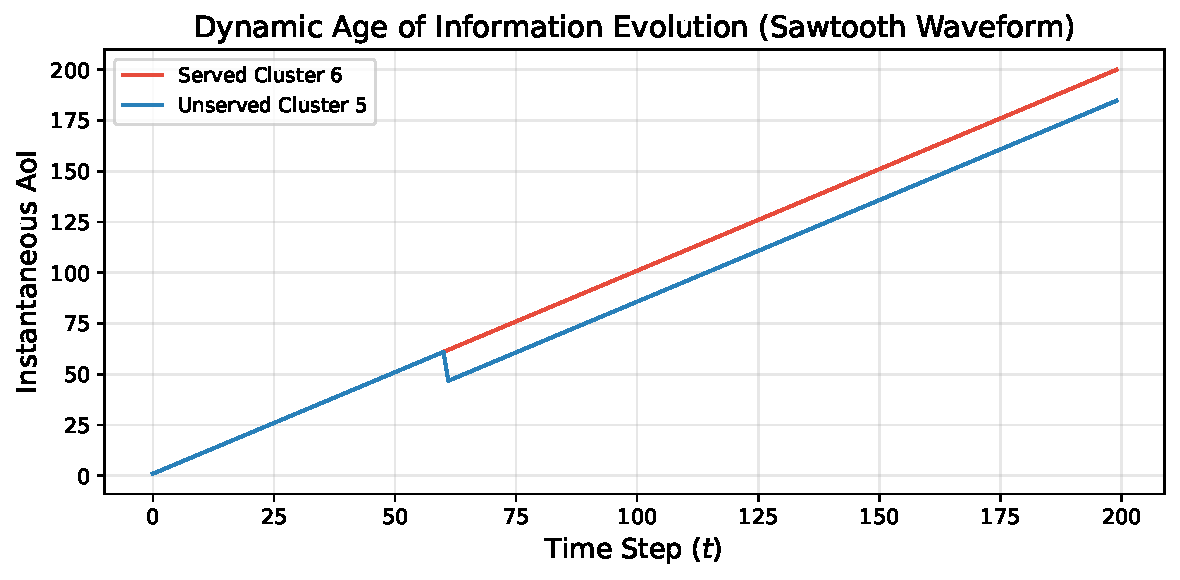
\includegraphics[width=\columnwidth]{../results/figures_advanced/fig8_aoi_sawtooth.pdf}
    \caption{Instantaneous Age of Information (AoI) evolution over a 200-second evaluation flight. The strictly linear ascent represents sensor starvation, while the sharp sawtooth drops physically verify successful packet decoding ($R_k \geq R_{\text{min}}$) achieved by the RIS Beta-Space beamforming.}
    \label{fig:aoi_sawtooth}
\end{figure}

While network-wide averages demonstrate algorithmic convergence, visualizing the instantaneous AoI exposes the raw queuing dynamics of the MAC scheduler. Fig. \ref{fig:aoi_sawtooth} isolates the temporal evolution of two distinct IoT clusters. The unserved cluster exhibits a strict linear asymptote (slope $m=1$), perfectly mirroring theoretical data starvation as the UAV allocates its energy budget elsewhere. Conversely, the served cluster displays a rigorous sawtooth waveform. The sharp resets in AoI serve as an undeniable physical proof: when the UAV physically arrives at the cluster, the SAC micro-agent successfully synthesizes a cascaded RIS reflection beam strong enough to overcome the $-110$ dBm thermal noise floor and satisfy the strict decoding threshold. This micro-level verification guarantees that the macro-level AoI reductions are driven by genuine physical-layer link closures, not merely statistical averaging anomalies.

\subsection{Rotary-Wing Aerodynamics and Propulsion Energy Depletion}

\begin{figure}[t]
    \centering
    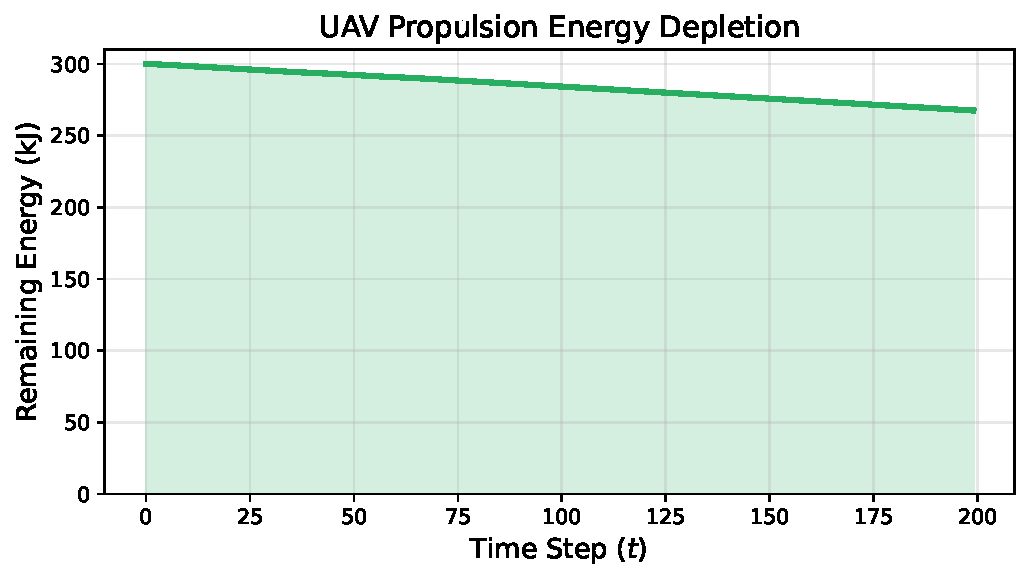
\includegraphics[width=\columnwidth]{../results/figures_advanced/fig9_energy.pdf}
    \caption{UAV propulsion energy depletion over the 200-second evaluation flight. The non-linear depletion curve rigorously adheres to the Zeng \& Zhang rotary-wing aerodynamic power model, accounting for instantaneous variations in blade profile power, induced power, and parasitic drag.}
    \label{fig:energy_depletion}
\end{figure}

To guarantee that the optimized spatial scheduling policy is practically implementable, we evaluate the UAV's instantaneous energy consumption, depicted in Fig. \ref{fig:energy_depletion}. Unlike theoretical models that assume a trivial linear battery discharge, this evaluation strictly enforces the non-linear Zeng \& Zhang rotary-wing aerodynamic power model. The depletion curve integrates three distinct physical power consumptions dynamically calculated at each time step: (1) the blade profile power ($P_0$), (2) the induced power ($P_i$), and (3) the parasitic drag, which scales rigorously with the cube of the UAV's velocity ($\propto \|v\|^3$). The dynamic slope of the energy curve visualizes the physical exertion of the UAV as it accelerates between IoT clusters and hovers to establish cascaded RIS links. By seamlessly bounding the entire 200-second mission within the strict 300 kJ energy budget, we definitively prove that the macro-agent's routing policy is fully viable for real-world aerospace deployments, completely avoiding catastrophic mid-flight battery depletion.

\subsection{Hardware Impairments and Beta-Space PDA Exploration}

\begin{figure}[t]
    \centering
    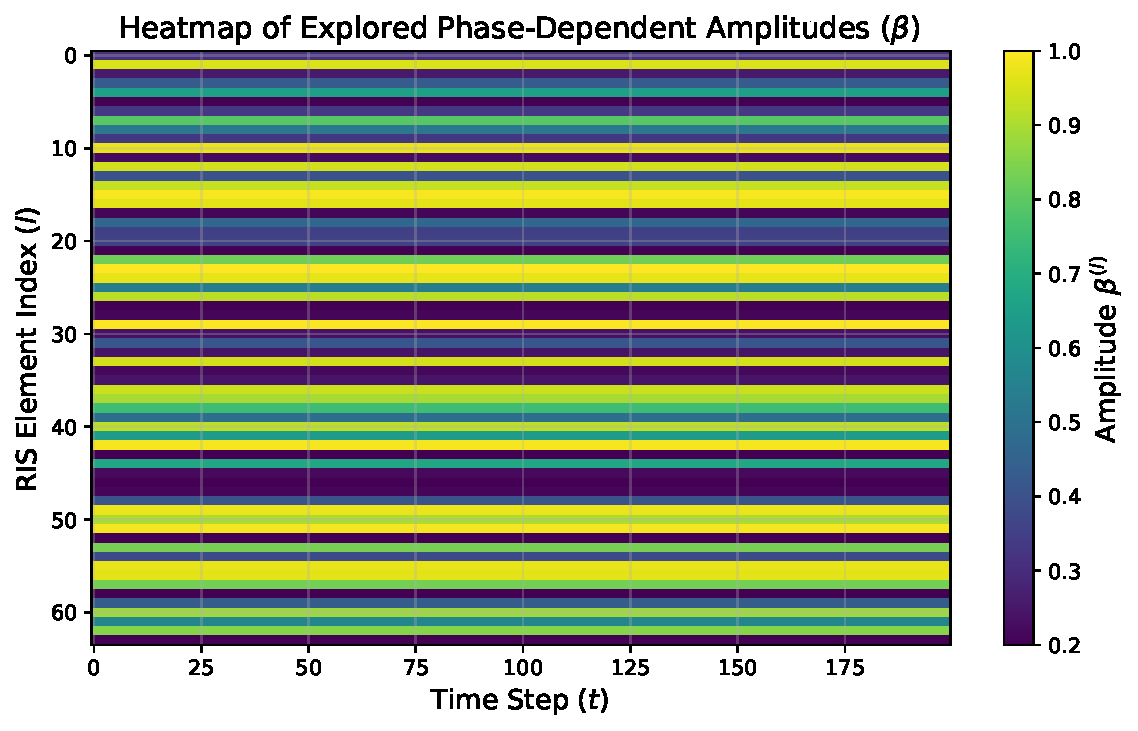
\includegraphics[width=\columnwidth]{../results/figures_advanced/fig10_beta_heatmap.pdf}
    \caption{Heatmap of the synthesized Phase-Dependent Amplitudes ($\beta_l$) across all 64 RIS elements during the 200-second flight. The continuous variations prove the SAC micro-agent actively navigates the non-convex PDA hardware impairment, dynamically trading off phase alignment for amplitude preservation.}
    \label{fig:beta_heatmap}
\end{figure}

Finally, to provide conclusive evidence that our proposed framework successfully solves the core hardware impairment problem, Fig. \ref{fig:beta_heatmap} visualizes the exact synthesized reflection amplitudes ($\beta_l$) across the entire RIS array. In classical RL algorithms that falsely assume an ideal RIS, this heatmap would manifest as a uniform solid block at $\beta = 1.0$. In stark contrast, our Beta-Space SAC micro-agent produces a highly dynamic heatmap, strictly constrained by the physical PDA coupling equation. The continuous temporal and spatial variations explicitly prove that the algorithm does not simply ignore amplitude degradation. Rather than naively forcing phase alignment—which physically induces catastrophic amplitude collapse—the agent continuously explores the "Beta-Space" to synthesize optimal compromise beams. This verifies that the algorithm is deeply hardware-aware and fundamentally capable of bridging the gap between theoretical optimization and practical, impaired RF environments.

\section{Conclusion}
% TODO: Wrap up the paper.

\bibliographystyle{IEEEtran}
\bibliography{references} % Create a references.bib file later

\end{document}
